\cut{
\begin{itemize}
\item Compiler
  \begin{itemize}
  \item Camlp4, tcc, and fmlc (generate typedefs and prefeed defs) 
  \end{itemize}

\item Runtime system
  \begin{itemize}
  \item data structure of feed items: iData, meta data, etc
  \item implementation of feed/stream: lazy list
  \item fetching mechanism: eager fetching vs. lazy consumption, 
    http\_client library, batch fetching
  \item parse using padsML easy lib
  \item concurrency
  \item error handling
  \item discussion of selected combinators: local pairing, 
    dependent pairing (separate thread/queue)
  \end{itemize}

\item Tools library
  \begin{itemize}
  \item use of generic tool framework and feeds runtime lib
  \item use of several external ocaml libs: rrdtools, xml\_light
  \end{itemize}

\item Future work (shall we include???)
  \begin{itemize}
  \item expose meta data to the surface language
  \item a second (simplified) prefeed def with type defs only
  \end{itemize}

\item Experiments
  \begin{itemize}
  \item performance metrics: throughput, network/system latency
  \item setup (mac powerbook g4, 100Mb ethernet connection, 
    comon spec, comon nodes, random selection of nodes)
  \item two tables and graphs: throughput peaks at 
    200 nodes (chunk size), sys latency almost constant,
    system is scalable to comon (842 nodes)
  \end{itemize}
\end{itemize}
}

The implementation of the \padsd{} system comes in
three parts: the compiler, the runtime system, and the
built-in tools library. In this section, we briefly
analyze these three parts, and present 
an evaluation of the system performance.  We conclude
with a discussion of our choice to design a language
extension to O'Caml as opposed to just a library.
%We will show that the system can easily scale
%to support PlanetLab-sized applications with 
%hundreds of nodes. 

\subsection{The Compiler}
There are two parts to the \padsd{} compiler:
(1) \cd{tcc}, the tool configuration compiler for .tc files, 
and (2) \cd{fmlc}, the
compiler of the feed declarations (.fml files). Both compilers
convert their sources into O'Caml, which is compiled and
linked to the run-time libraries.  Each tool was implemented using 
Camlp4, the O'Caml preprocessor. 

\begin{figure}[t]
\centering
\begin{codebox}
let simple_comon =
\{\kw{frep} = fun ff ->
 ff.\kw{all}
 \{Combinators.\kw{format} = Comon_format.Source.parse;
  \kw{print} = Comon_format.Source.print;
  \kw{format_rep} = Comon_format.Source.tyrep; 
  \kw{incremental} = false;
  \kw{header_format} = None; 
  \kw{locations} = sites;
  \kw{schedule} =
    Schedule.{\kw every} (Time.now (), 10., 
                    Schedule.default_duration, 60.);
  \kw{has_records} = Comon_format.__PML__has_records; 
  \kw{pp} = None\}\}
\end{codebox}
\caption{Code snipet of compiled simple\_comon feed}\label{fig:compiledcomon}
\end{figure}

%A source program is parsed into an abstract
%syntax tree defined by the Camlp4 extended syntax, and the
%code generation is done through the quotation system. 
In the case of \cd{fmlc}, code generation is performed in two steps.
In the first step, the code generator emits a collection of
necessary type declarations for each feeds, while in the second step
it generates representations of the feed descriptions.  These representations
are coded by extracting various elements from the concurrently
compiled \padsml{} libraries,
and using a collection of polymorphic combinators to build structured 
descriptions.  Figure \ref{fig:compiledcomon} shows a fragment of
the compiled code for
the simple CoMon feed in Figure \ref{fig:simplecomon}.
While a programmer could use our combinator library directly, the
surface syntax provides a simple veneer that reduces the barrier to
entry substantially.
% in a
%lazy fashion (that is, only generate the declaration if the
%feed is used in the rest of the description).
%In the second step, 
%,
%also known as the ``prefeed''. Schedules which are
%definite times such as ``2008/09/30:12:00:00'' or ``5 mins'' are
%converted to floating point number of seconds at compile time
%to make the code more efficient.
%All O'Caml expressions embeded in the fml file are
%included without change in the compiled code. 

\subsection{The Run-time System}
A feed in \padsd{} is implemented as a lazy list of feed
items. 
Following the semantics presented in Section~\ref{sec:semantics}, 
a feed item is a metadata/data pair,
though the implementation's meta-data records contain additional information
such as data arrival times and more detailed error codes. 
Some of these error codes include miscellaneous HTTP error, late item
arrival, parse error, etc.

% Late arrival, (3)
% %{{\small{ 
% \begin{verbatim}
% 1: Misc HTTP error
% 2: Late arrival
% 3: Ssh host required
% 4: Remote command required for ssh
% 5: Bad message
% \end{verbatim}
% %}}} \normalsize

% % This means the feed 
% % is actually a function {\tt next}. It is evaluated 
% % only when the user program attempts to take an
% % item from the feed. The function {\tt next} returns an
% % item plus a new {\tt next} function which represents
% % the tail of the feed.
% %a data item of polymorphic type 'a and 
% %a meta data structure that corresponds 'a. 
% %The type of a feed is also the type of its data item. 
% %The type of a base feed has an option type.
% The meta data is a tree structure in which
% each node is tagged with a meta header. 
% The tree structure (also known as the meta body) resembles 
% the structure of the data item, i.e.  if the data item is a pair, 
% then the meta body is also a pair of meta data. Each leaf
% of the meta body corresponds to a base feed. Meta information
% such as the scheduled time, arrival time, location and 
% errors is stored in the leaves. The header records the summary 
% of meta information within the subtree. 

The \padsd{} runtime system is a multi-threaded concurrent
system composed that uses a master-worker implementation strategy. 
%Each base feed is created and maintained by a separate 
%worker thread, and a master thread drives the combination of 
%base feeds into compound feeds.  
Each worker thread either fetches data from the specified
location and parses the data into an internal representation (the {\em rep})
%(known as the {\em rep})
using the \padsml{} parser, or synthesizes its data by calling some 
generator function.  Using error conditions, location, scheduled
and arrival times, the worker generates the appropriately shaped metadata,
pairs it with the rep and pushes the feed item onto a queue. 
%And then it generates the idata from the rep and the meta data,
%and pushes the idata into the concurrent queue.
%The workers communicated with
%the master through a concurrent queue.
The master thread pops the feed item from the queue on demand --- that is,
when the data is requested by the user program. In other words,
the worker thread is {\em eager}, which guarantees all potentially 
necessary data will be fetched and archived, but the master thread is 
{\em lazy}, allowing application programs to process only the data they
need at their whim.
%The concurrency control is implemented by the O'Caml threads
%library using standard mutex and condition variables.

The fetching engine is implemented using
the Ocamlnet 2 library~\cite{ocamlnet2}. 
%which is capable of concurrent fetches. 
Given a list of locations to fetch from at any one time, 
the system converts the list into batches and fetches up to 200 locations
per batch. The choice of 200 is a trade-off between maximizing
the throughput and avoiding overwhelming the operating system
with too many open sockets. 
%If the system fails to fetch an
%item due to network or system error, a feed item is still created
%with the appropriate error code written in the metadata. 

% The \padsd{} system does not 
% automatically filter out erroneous items because errors often 
% provides very important information to users who monitors 
% distributed systems. Users could optional choose to filter
% out bad feed items using the Feed library functions.

% Compound feeds are created within the generic tool framework by
% combining base feeds using various combinator functions.
% These functions takes idatas from two feeds and creates a new idata often
% by comparing the timestamps in the two idatas. While this is done
% lazily in most of the combinators, it is not the case for
% dependent pairs. This is because the dependent feed needs to be
% created {\em eagerly} when each item from the {\em depending}
% feed arrives. Therefore we add another layer of ``pseudo-fetching"
% for the dependent feed. Here a separate thread is created for each
% dependent feed, which actively takes data from the depending
% feed, creates dependent items, and push to another concurrent
% queue of its own.  
 
\subsection{Tools Library}
As explained in Section~\ref{sec:programming},
the quick-and-dirty tool suite was implemented using the
generic tools framework.  Many of the tools rely upon
format-specific library is generated at compile time by the underlying
\padsml{} compiler.  For instance, the feed selector relies upon 
a selector generated by type-directed compilation of the \padsml{}
description.  Other tools depend upon auxiliary libraries.
For instance, the feed2rrd tool requires the RRD round-robin 
database~\cite{rrdtool}
and the feed2rss tool uses the XML-Light package for parsing
and printing~\cite{xmllight}.
%The system also provides an Feed interface to a number of
%useful runtime functions such as map and fold for advanced
%users to program against the feeds.

\cut{
\begin{table*}[th]
\begin{center}
\begin{tabular}{|l|r|r|r|r|r|r|r|r|r|r|r|r|}\hline
Num of nodes&	50&	100&	150&	200&	250&	300&	350&	400&	450&	500&	550&	600 \\ \hline\hline
Net latency per node (secs)&	9&	4&	4&	4&	8.6&	5.3&	19.1&	19.5&	14.4&	7.8&	12&	13.3 \\ \hline
Sys latency per node (secs)&	0&	0&	0&	0.3&	0.2&	0.4&	0.3&	0.1&	0.3&	0.4&	0.2&	0.7 \\ \hline
%Total Latency (secs)&	9&	4.04&	4&	4.3&	8.8&	5.8&	19.4&	19.6&	14.7&	8.2&	12.3&	14 \\ \hline
Total fetch time (secs)&	9&	5&	4&	5&	23&	9&	22&	23&	26&	14&	27&	28 \\ \hline	
Throughput (items/sec)&	5.6&	20&	37.5&	40&	10.9&	33.3&	15.9&	17.4&	17.3&	35.7&	20.4&	21.4 \\ \hline
\end{tabular}
\end{center}
\caption{Performance of CoMon without archiving}
\label{tab:comon-noarch}
\end{table*}


\begin{table*}
\begin{center}
\begin{tabular}{|l|r|r|r|r|r|r|r|r|r|r|r|r|}\hline
Num of nodes&	50&	100&	150&	200&	250&	300&	350&	400&	450&	500&	550&	600 \\ \hline\hline
Net latency per node (secs)&	16&	4&	4&	4&	18.9&	6&	20.6&	22&	8.4&	13&	21.8&	21.3 \\ \hline
Sys latency per node (secs)&	0.8&	1.28&	1.4&	1.8&	1.9&	1.5&	1.6&	1.3&	1.9&	1.7&	1.7&	2.2 \\ \hline
%Total Latency (secs)&	16.8&	5.28&	5.4&	5.8&	20.8&	7.5&	22.2&	23.3&	10.3&	14.7&	23.56&	23.5 \\ \hline
Total fetch time (secs)&	17&	6&	7&	7&	27&	12&	27&	30&	19&	33&	43&	43 \\ \hline
Throughput (items/sec)&	2.9&	16.7&	21.4&	28.6&	9.3&	25&	13&	13.3&	23.7&	15.2&	12.8&	14 \\ \hline
\end{tabular}
\end{center}
\caption{Performance of CoMon with archiving}
\label{tab:comon-arch}
\end{table*}
}

\subsection{Experiments} \label{sec:experiments}

\begin{figure}[t]
\begin{center}
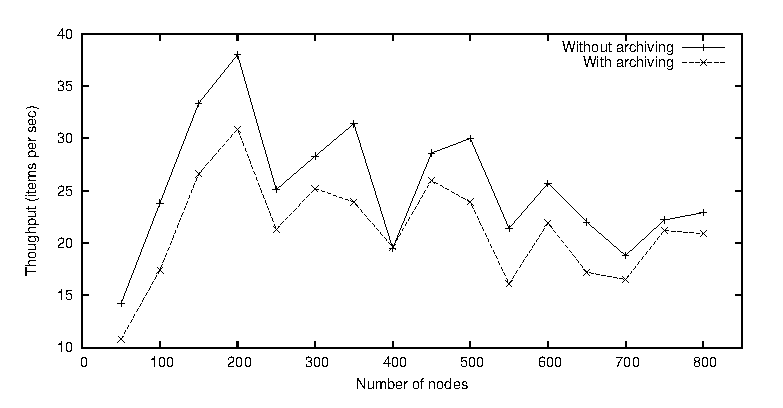
\epsfig{file=throughput.eps, width=\columnwidth}
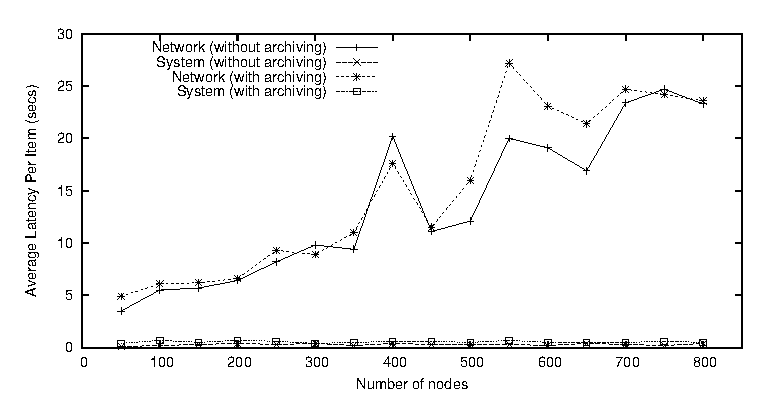
\epsfig{file=latency.eps, width=\columnwidth}
\caption{Average throughput and latencies per node}
\label{fig:throughput}
\end{center}
\end{figure}

To assess system performance,
we measure the average network latency
to fetch a data item, the average system latency 
to produce a data item
and the throughput of the system using the CoMon feed
description in Figure \ref{fig:feedcomon}. 
The throughput measures the average
number of items fetched per second. 
%We picked
%the comon example because it is a real life
%application that involves fetching from large number of 
%nodes (800+) at the same time, which can be viewed as a stress test. 

All the experiments were conducted on a Mac Powerbook G4 computer
with a 1.67GHz CPU and 2GB memory running Mac OS X 10.4. It is
connected to the internet via a 11Mb/s wireless ethernet.
In each experiment, We randomly selected 50 nodes,
100 nodes, up to 800 PlanetLab nodes
%\footnote{List taken from http://www.cs.princeton.edu/~vivek/node\_list\_all. 
%Nodes could come and go sporadically.} 
to form
16 node sets. For each node set,
we applied the profiler tool on the comon feed twice, one without
archiving and one with archiving, and measured the throughput
and latencies as the system fetched from these node lists. 
We then repeat the experiment ten times and calculate the average values.

Figure \ref{fig:throughput} shows the average throughtput
and the average network and system latencies measured.
Generally, 
%the throughtput goes up with the number of nodes
%until 200 and then starts declining and saturating
%as it approaches 800. Locally, 
the throughput hits peaks at
multiples of 200 nodes since the system supports 
200 concurrent fetches at one time.
%is the size of the
%fetching batch. At multiples of 200, the concurrent
%fetching is maximally utilized. 
An anomaly occurred 
%The exception is
at 400 nodes, as 
%the node sets contain 
a number nodes were unreachable due to DNS failures.
% at the time of
%the experiment. 
%It is also noted that
%archiving adds to the overhead of the system and hence
%reduces the throughput. 
When analyzing latency, the main message is that
while network latency goes up with the number of nodes,
the system latency remains almost constant and relatively
small. This shows that the \padsd{} runtime system adds
very little overhead to the inevitable network fetching
cost. It also worth noting that the network latency is
almost linear with the number of nodes. Overall, the system
could fetch from up to 800 nodes and archive all the data in under 
40 secs, which provides ample breathing room inside the 
5-minute turnaround time currently supported by 
CoMon. Taken together, these results suggest that the system is 
perfectly capable of supporting PlanetLab-scale monitoring applications. 

%Tables \ref{tab:comon-noarch} and \ref{tab:comon-arch}
%shows the results from two different scenarios:
%one in which the user program simply creates the comon feed without applying
%any tools on it, and one in which the comon feed is created
%and archived. In both scenarios, the system was
%able to fetch from up to 600 nodes within one minute, which is
%significantly shorter than the 5-minute turnaround time in the real
%CoMon system.
%\begin{figure}[th]
%\begin{center}
%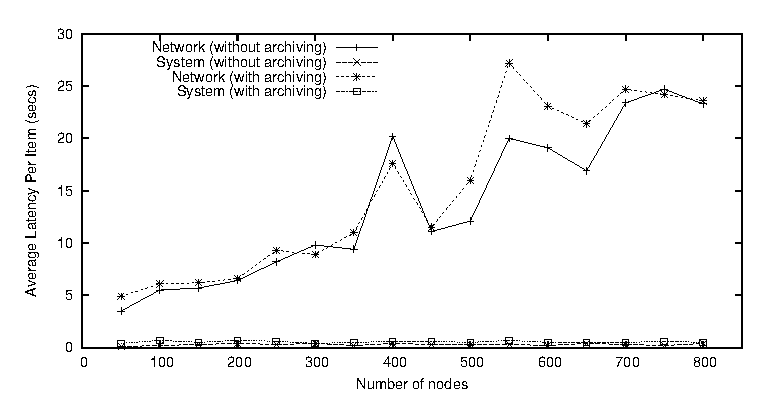
\epsfig{file=latency.eps, width=\columnwidth}
%\caption{Average latencies per node}
%\label{fig:latency}
%\end{center}
%\end{figure}

\cut{
We plot the average throughput in Figure \ref{fig:throughput}
and the system and network latencies in Figure \ref{fig:latency}. 
As expected, both the thoughput and latency suffer a little with 
archiving taking place. The throughput peaks when fetching from
200 nodes because 200 is the size of the fetching batch and
at 200 nodes, the concurrent fetching engine is maximally utilized.
The experiment for 450 nodes exhibits an anomaly as the archived
experiment takes less time than the un-archived experiment.
This is probably due to sudden delays in some of the nodes when the
no-archiving experiment is run. One obvious take-away from
Figure \ref{fig:latency} is that while the network latency may
vary greatly depending on the network condition, the system latency
stays almost constant at relatively low levels. This shows that
the \padsd{} system runtime adds little overhead to the 
inevitable network cost, which means the system could scale to
large applications. 
}

\subsection{Language or Library?}

% reason (4) managing functors & modules?

Our language of feeds is a relatively thin veneer on top of O'Caml
implemented by the Camlp4 preprocessor.  
Hence, a natural question to ask is whether the system would be better
implemented as a library as opposed to a language extension with its
own syntax and code generator.  There are three main reasons we chose
to present our work as a language.
\begin{enumerate}
\item {\bf Automatic elimination of boilerplate code.} Much of the boilerplate 
elimination is achieved by parsing fml and config files, filling in 
defaults and automatically generating driver programs for the naive 
user that string together generic tools.  Other boilerplate is avoided
by generating both types and values automatically from descriptions
(particularly datatype descriptions) and packaging them inside modules.
\item {\bf Simplicity of coding style for the quick-and-dirty user.}  Our
Mogensen-Scott encodings, for example, while 
palatable for the advanced functional programmer, involve {\em very}
higher-order interfaces with unusually complicated types and heavy
use of the module system.  It simply seems more involved than the 
average computational biologist is willing to stomach.
\item {\bf Lack of convenient support for generic programming in O'Caml.} As mentioned
previously, many of the tools and libraries are type-directed programs, 
the implementation of which requires set up of complex higher-order 
data structures with unusual types more easily generated automatically
than programmed directly. 
\end{enumerate}
Having made our case for a language extension, the bulk of our implementation
{\em is} a collection of libraries.  Hence, the intrepid hacker may eschew our
surface syntax and program directly against the interfaces underneith.
Whatever the programmer chooses, the central contribution of this work
are the abstractions we provide.  Moreover
by defining a compact calculus of feeds with a precise formal
semantics, we believe the ideas presented in this paper can transcend
their current implementation.  We would be thrilled if others would
take our abstractions and embed them directly in another language,
such as Haskell, that provides superior generic programming support
and the ability to automatically derive implementations from appropriately
specified type classes.
